\section{Amplitude modulation : Vestigial Sideband (VSB)}
Vestigial sideband (VSB) is a type of amplitude modulation ( AM ) technique (sometimes called VSB-AM ) that encodes data by varying the amplitude of a single carrier frequency . Portions of one of the redundant sidebands are removed to form a vestigial sideband signal - so-called because a vestige of the sideband remains.
VSB transmission is similar to single-sideband (SSB) transmission, in which one of the sidebands is completely removed. In VSB transmission, however, the second sideband is not completely removed, but is filtered to remove all but the desired range of frequencies .
\subsection{Modulation:}
This means that the use of SSB modulation is inappropriate for the transmission of such message signals owing to the practical difficulty of building a filter to isolate one sideband completely.
This difficulty suggests another scheme known as vestigial sideband modulation (VSB), which is a compromise between SSB and DSB-SC forms of modulation. In VSB modulation, one sideband is passed almost completely whereas just a trace or vestige, of the other sideband is retained. Figure \ref{fig:1} illustrates the spectrum of a VSB modulated wave s(t) in relation to that of the message signal m(t) assuming that the lower sideband is modified into the vestigial sideband.

\begin{equation}
    \Phi_{VSB}(f) = [M(f+f_c) + M(f-f_c)]H_i(f)
\end{equation}

\begin{figure}[h!]
    \centering
    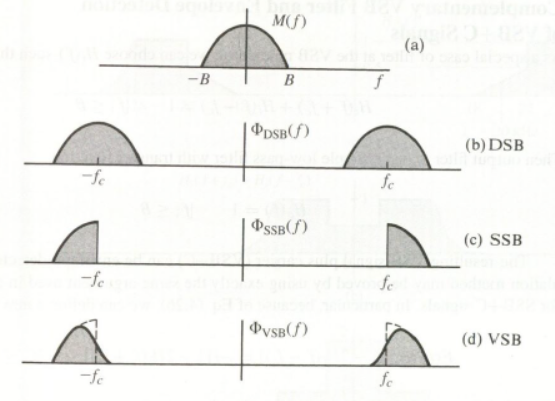
\includegraphics{figures/fig_1.png}
    \caption{}
    \label{fig:1}
\end{figure}
\begin{figure}[h!]
    \centering
    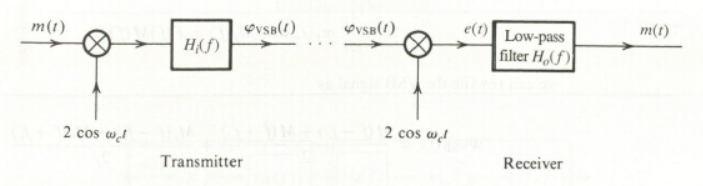
\includegraphics{figures/fig_2.png}
    \caption{}
    \label{fig:2}
\end{figure}

\subsection{Demodulation:}

We require that  $m(t)$ is recoverable from $\phi(t)$ using synchronous demodulaton at the receiver. This is done multiplying $\phi(t)$ by $2cos(\omega t)$. The product e(t) given by
\begin{equation}
    e(t) = 2\phi_{VSB}(t)cos(\omega_ct) <=> [\Phi_{VSB}(f+f_c) + \Phi_{VSB}(f-f_c)]
\end{equation}
The signal e(t) is passed through low pass equalizer filter  of transfer function H0(f). The output of the filter is required to be m(t). So output spectrum will be
\begin{equation}
    M(f) = [\Phi_{VSB}(f+f_c) + \Phi_{VSB}(f-f_c)]H_o(f)
\end{equation}
Substituting equation into this equation and eliminating the spectra at $+-2f_c$ by a low pass filter $H_o(f)$, we obtain
\begin{equation}
    M(f) = M(f)[H_i(f+f_c) + H_i(f-f_c)]H_o(f)
\end{equation}
Hence
\begin{equation}
    H_o(f) = \frac{1}{H_i(f+f_c) + H_i(f-f_c)}
\end{equation}

\section{PHASE-LOCKED LOOP (PLL)}
The phase lock loop is a very important device used to track the phase and the frequency of the carrier component of an incoming signal. A PLL has three basic components

\begin{itemize}
    \item A voltage control oscillator (VCO)
    \item A multiplier, serving as a phase detector (PD)
    or phase comparator
    \item A loop filter H(s)
\end{itemize}

Only phase change:
\begin{equation}
    \begin{split}
        Asin(\omega_ct+\theta_i) * Bcos(\omega_ct+\theta_o)\\
        =\frac{AB}{2}[sin(2\omega_ct+\theta_i+\theta_o) + sin(\theta_i-\theta_o)]\\
    \end{split}
\end{equation}
here, $sin(2\omega_ct+\theta_i+\theta_o)$ is being filter out \\
Remaining portion
\begin{equation}
    \frac{AB}{2}sin(\theta_i-\theta_o)]
\end{equation}

Demodulation for DSB-SC:
\begin{equation}
    \begin{split}
        m(t)[cos(\omega_ct) * 2cos((\omega_c+\Delta\omega)t+\theta)]\\
        =m(t)[cos(2\omega_ct+\Delta\omega t+\theta) + cos(\Delta\omega t+\theta)]
    \end{split}
\end{equation}
here, $cos(2\omega_ct+\Delta\omega t+\theta)$ is being filter out \\
Remaining portion
\begin{equation}
    m(t)cos(\Delta\omega t+\theta)]
\end{equation}

Impact of phase difference\\
Let $\Delta\omega$ be 0, then we have
\begin{equation}
    m(t)cos(\theta)]
\end{equation}

Impact of frequency difference\\
Let $\theta$ be 0, then we have
\begin{equation}
    m(t)cos(\Delta\omega t)]
\end{equation}
